%!TEX root = Intro-NLP-seminar.tex
\section{NLP Processing Layers}

\begin{frame}
\frametitle{Linguistic Layers in NLP}

\centering

\begin{tabular}{c @{ $\Longleftrightarrow$ } c}
Morphology & word formation\\
Syntax & sentence structure, grammar\\
Semantics & meaning\\
Pragmatics & discourse, context\\[1em]
Speech & phonemes (speech units)
\end{tabular}

\end{frame}

\plain{Examples here are for English -- other languages may need different approaches}


\subsection{Morphology}

\begin{frame}
\frametitle{Morphology}
\begin{itemize}[<+->]
	\item How words are formed
		\begin{description}[Derivation:]
			\item[Inflection:] plant $\longrightarrow$ plants, planted, planting \ldots 
			\item[Derivation:] plant $\longrightarrow$ plantation, implant \ldots
		\end{description}
	\item For Malay:
		\begin{description}[Derivation:]
		\item[Inflection:] sakit $\longrightarrow$ sakitnya; pergi $\longrightarrow$ pergilah
		\item[Derivation:] sakit $\longrightarrow$ pesakit, penyakit, sakitan\ldots
		\end{description}
	\item Morphology processing: related to words
\end{itemize}
\end{frame}


\begin{frame}
\frametitle{Tokenising}

\begin{itemize}[<+->]
	\item Split input text into processable units
	\item Just by space characters\ldots?
		\begin{itemize}
			\item 
			\tikz[baseline, start chain=going right, node distance=0.5em, every node/.style={on chain, draw, text height=1.25ex, text depth=.25ex}]
			\path node{Passers-by} node{didn't} node{go} node[draw=none]{\ldots};
		\end{itemize}
	\item Just by punctuation/word boundaries\ldots?
		\begin{itemize}
			\item \tikz[baseline, start chain=going right, node distance=0.5em, every node/.style={on chain, draw, text height=1.25ex, text depth=.25ex}]
			\path node{Passers} node{-} node{by} node{didn} node{'} node{t} node{go} node[draw=none]{\ldots};
		\end{itemize}
	\item \alert{Tokenizers need to consider natural language!}
		\begin{itemize}
			\item \tikz[baseline, start chain=going right, node distance=0.5em, every node/.style={on chain, draw, text height=1.25ex, text depth=.25ex}]
			\path node{Passers-by} node{did} node{n't} node{go} node[draw=none]{\ldots};

		\end{itemize}
\end{itemize}

\end{frame}


\begin{frame}
\frametitle{Sentence Splitting}
\begin{itemize}
	\item How to identify sentence boundaries?
	\item ``That's wonderful,' he said. `Have your people call mine. Try to arrange something by 10 a.m. tomorrow.''
\end{itemize}
\end{frame}


\begin{frame}[allowframebreaks]
\frametitle{Stemming}
    
\begin{itemize}
\item \textbf{Stem:} reduced form (word stem, base or root form) or a word
\item Need not be identical to the morphological root of the word!
\item As long as related words map to the same stem
\item Usually implemented by stripping prefix/suffix

\framebreak

\item Example stemming:
	\begin{itemize}
	\item carresses $\rightarrow$ carress
	\item ponies $\rightarrow$ poni
	\item caress $\rightarrow$ caress
	\item cats $\rightarrow$ cat
	\item producer $\rightarrow$ produc
	\item produced $\rightarrow$ produc
	\item producing $\rightarrow$ produc
	\end{itemize}

\item Can have phases/sequences of rules \parencite{porter:1980,paice:1994}
\end{itemize}

\end{frame}

\begin{frame}
\frametitle{Why Stemming?}
    
\begin{itemize}[<+->]
\item Information Retrieval -- search for documents based on keywords
\item Stem all words in documents and store as index
\item Input keyword: producer $\rightarrow$ `produc'
\item Search documents whose indices contain `produc'
\item Results will include documents containing `produce', `produced', `producer' \ldots
\end{itemize}

\end{frame}


\begin{frame}[allowframebreaks]
\frametitle{Lemmatising}

\begin{itemize}
\item \textbf{Lemma:} base form of a word or term that is used as the \emph{formal dictionary entry} for the term.
\item Lemmatising can be seen as a special form of stemming
	\begin{itemize}
	\item Stemming: outputs do not need to be real words
	\item Lemmatising: outputs are genuine words used as headwords in dictionaries
	\end{itemize}
\end{itemize}

\ex
\begingl
\gla \textsmaller{Input:} banks raised rates to fight inflation//
\glb \textsmaller{Lemmas:} bank raise rates to fight inflation//
\endgl
\xe
\end{frame}


\begin{frame}
\frametitle{Stemming vs Lemmatising}
    
\begin{itemize}
\item Stemming is much faster than lemmatising
\item But lemmatising is essential for many NLP tasks
\end{itemize}

\end{frame}

\begin{frame}
\frametitle{Would lemmatising be required for these languages?}

\begin{itemize}
\item Malay
\item Chinese
\end{itemize}

\end{frame}


\begin{frame}
\frametitle{Segmentation}
\begin{itemize}[<+->]
\item Languages without word boundaries, e.g.~Chinese, Thai, Japanese, German\ldots
\item Essential for proper understanding!
\item Chinese example: {\xiheifont 有职称的和尚未有职称的}

\ex
\xiheifont
\begingl
\gla 有 职称 的 和 尚未 有 职称 的//
\glb with position ones and {not yet} with position ones//
\endgl
\xe

\ex
\xiheifont
\begingl
\gla 有 职称 的 \alert{和尚} 未有 职称 的//
\glb with position ones \alert{monks} without position ones//
\endgl
\xe

\end{itemize}

\end{frame}


\begin{frame}
\frametitle{Technological readiness}
    
\begin{itemize}
\item For English: libraries exists to perform these tasks
\item For other languages: depends -- some are still under research and development
\end{itemize}

\end{frame}

\subsection{Syntax}

\begin{frame}
\frametitle{Syntax}
\begin{itemize}
\item How words \emph{form phrases and sentences}
\item Grammatical rules and structures!
\item Syntactic processing: extract structure of phrase/sentences
\end{itemize}
\end{frame}


\begin{frame}[allowframebreaks]
\frametitle{Part-of-Speech (POS)}

\begin{itemize}[<+->]
\item A category assigned to a word based on its grammatical and semantic properties.
\item Example: noun, verb, adjective, adverb, determiner, preposition\ldots
\item Different languages may have different sets of POS e.g.~classifier (penjodoh bilangan)
%\item Open-class words (content words): nouns, verbs, adjectives, adverbs
%\item Closed-class words (function words): determiners, pronouns, conjunctions, infinitives\ldots
\end{itemize}
\end{frame}

\begin{frame}
\frametitle{POS Tagset}
\begin{itemize}
\item English: Penn Treebank (PTB) tagset is widely adopted \parencite{marcus1993building}
\item \url{https://www.ling.upenn.edu/courses/Fall_2003/ling001/penn_treebank_pos.html}
\end{itemize}
 
\begin{center}
\begin{tabular}{ll}
\toprule
Tag & Description\\
\midrule
NN & Noun, singular or mass\\
NNS & Noun, plural\\
VB & Verb, base form\\
VBD & Verb, past tense\\
VBG & Verb, gerund or present participle\\
\ldots & \ldots\\
\bottomrule
\end{tabular}
\end{center}

\end{frame}


\begin{frame}
\frametitle{POS-tagging}
    
\begin{itemize}
\item Given an utterance, assign the most likely POS tag to each word token
\item Current libraries quite stable now (for English): $\sim 96\%$ accuracy
\end{itemize}

\ex\deftagex{basic}
\begingl
\gla \textsmaller{Input:} banks raised rates to fight inflation//
\glb \textsmaller{POS-tags:} NNS VBD NNS TO VB NN//
\endgl
\xe 

\end{frame}


\begin{frame}
\frametitle{Phrase and Sentence Structure}
    
\begin{itemize}[<+->]
\item Sentences/clauses are made up of \emph{phrases} following grammar (syntax) rules
\item Some examples:
\begin{itemize}
\item Noun phrase (NP): `a bright star', `cats', `stars and moons'
\item Verb phrase (VP): `ran', `pick the ball up'
\item Clause/sentence (S): NP VP `a bright star pick the ball up'
\end{itemize}
\item (A syntactically correct sentence doesn't guarantee it makes sense!)
\end{itemize}

\end{frame}


\begin{frame}[fragile]
\frametitle{Shallow parsing (chunking)}

\begin{itemize}

\item Identify the noun phrases, verb phrases etc but do not go into the internal structure

\begin{multicols}{2}
\begin{tikzpicture}[transform shape, scale=.8]
\Tree [.S [.NP \edge[roof]; banks ] 
	[.VP \edge[roof]; {raised rates} ] 
	[.VP \edge[roof]; {to fight inflation} ]
]
\end{tikzpicture}

\pause
\begin{tikzpicture}[transform shape, scale=.8]
\Tree [.S [.NP \edge[roof]; {A bright star} ] 
	[.VP \edge[roof]; {pick the ball up} ] 
]
\end{tikzpicture}

\end{multicols}

\end{itemize}
\end{frame}

\begin{frame}[fragile]
\frametitle{Parsing (deep parsing)}

\begin{itemize}
\item Fully building the clauses and relations in a sentence
\item Syntactic parse tree:
\begin{multicols}{2}
`Banks raised rates to fight inflation'

{\small
\begin{verbatim}
(S
  (NP (NNS banks))
  (VP (VBD raised)
    (NP (NNS rates))
    (S
      (VP (TO to)
        (VP (VB fight)
          (NP (NN inflation)))))))
\end{verbatim}
}

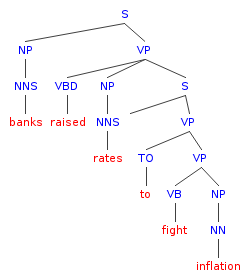
\includegraphics[width=\linewidth]{syntax-tree}

\end{multicols}
\end{itemize}
\end{frame}


\begin{frame}[fragile]
\frametitle{Dependency parsing}

\begin{itemize}
\item Find dependency relations in the text
\end{itemize}

\begin{multicols}{2}
`Banks raised rates to fight inflation'

{\small
\begin{verbatim}
nsubj(raised, banks)
root(ROOT, raised)
dobj(raised, rates)
aux(fight, to)
vmod(raised, fight)
dobj(fight, inflation)
\end{verbatim}
}

\begin{tikzpicture}[transform shape]
\Tree [.raised 
	banks
	rates
	[.fight to inflation ]
]
\end{tikzpicture}

\pause

\begin{itemize}
\item `banks' is subject of `raised'
\item `rates' is object of `raised'
\item \ldots
\end{itemize}

\end{multicols}

\end{frame}


\begin{frame}
\frametitle{Technological Readiness}
    
\begin{itemize}
\item Parsing is more difficult than POS-tagging
\item But largely solved for English
\item Varies for other languages (e.g.~OK for Chinese, no truly satisfactory one yet for Malay)
\end{itemize}

\end{frame}

\subsection{Semantic}

\begin{frame}
\frametitle{Semantic}

\begin{itemize}
\item The meaning conveyed by the text
\item Hard!
\item How to represent `meaning'?
\item Still an open question in articifial intelligence, cognitive science, psychology\ldots
\item Lots of on-going research
\end{itemize} 

\end{frame}


\begin{frame}
\frametitle{Word Sense}
    
\begin{itemize}
\item One of zero to many \emph{meanings or concepts} associated with a given \emph{head word/lemma}, as listed in a specific lexicon
\item Lexicon: a machine-readable, structured dictionary
\item May also include relations between word senses
	\begin{itemize}
	\item Synonyms, antonyms, is-a-type-of\ldots
	\end{itemize}
\end{itemize}

\end{frame}


\begin{frame}
\frametitle{Synonym Expansion}
    
\begin{itemize}
\item Example in information retrieval (search engine)
\item Search for `wizard' would also retrieve documents containing `sorcerer', `magician'
\end{itemize}

\end{frame}


\begin{frame}
\frametitle{Word Sense Disambiguation (WSD)}

\begin{itemize}
\item a.k.a.~Sense-tagging
\item Associating a word occurrence with its most likely sense, with repect to a specific lexicon
\item \textbf{Stop words:} Words that are ignored in NLP tasks, e.g.~function words in a sense-tagging task.
\end{itemize}
\end{frame}

\begin{frame}
\frametitle{How to identify stop words?}

\begin{itemize}
\item Open-class words (content words): nouns, verbs, adjectives, adverbs
\item Closed-class words (function words): determiners, pronouns, conjunctions, infinitives\ldots
\end{itemize}

\ldots so WSD needs POS-tagging and lemmatisation first

\end{frame}

\begin{frame}
\frametitle{WSD Example}

\begin{exampleblock}{Senses of bank.n in WordNet}
\begin{enumerate}
\item sloping land (especially the slope beside a body of water)
\item a financial institution that accepts deposits and channels the money into lending activities
\item a long ridge or pile
\item \ldots
\end{enumerate}
\end{exampleblock}

\ex\deftagex{basic}
\begingl
\gla \textsmaller{Input:} banks raised rates to fight inflation//
\glb \textsmaller{Sense-tags:} bank.n.2 raise.v.13 rates.n.1 {} fight.v.1 inflation.n.1//
\endgl
\xe     
\end{frame}


\begin{frame}
\frametitle{Concept Tagging}
    
\begin{itemize}
\item Label each sense in the input with a concept tag \\
(Example below uses WordNet--SUMO mapping)
\end{itemize}

\lingset{everyglb={\footnotesize}, everyglc={\scriptsize\scshape}}
\ex\deftagex{basic}
\begingl
\gla \textsmaller{Input:} banks raised rates to fight inflation//
\glb \textsmaller{Sense-tags:} bank.n.2 raise.v.13 rates.n.1 {} fight.v.1 inflation.n.1//
\glc \textsmaller{\upshape Concept tags:} Corporation Increasing Tax {}  ViolentContest Increasing//
\endgl
\xe 

\end{frame}


\begin{frame}
\frametitle{Information Extraction}

\begin{itemize}
\item Examples as given earlier
\item Named entity recognition
\item Coreference resolution
	\begin{itemize}[<+->]
	\item `The cat climbed onto the chair. It yawned and slept.'
	\item `It' = `the cat'? `the chair'?
	\item `cat' $\xrightarrow{\text{is-a}}$ \textsc{animal} $\xrightarrow{\text{is-a}}$ \textsc{animate object}
	\item `chair' $\xrightarrow{\text{is-a}}$ \textsc{furniture} $\xrightarrow{\text{is-a}}$ \textsc{inanimate object}
	\item \textsc{animate object} $\xrightarrow{\text{capable-of}}$ `yawn', `sleep'
	\item $\therefore$ `It' = `the cat'
	\end{itemize}
\end{itemize}

\end{frame}



\subsection{Pragmatics}

\begin{frame}
\frametitle{Pragmatics}

\begin{itemize}[<+->]
\item Processing text by inclduing context
\item Scenario, behavior, cultural, etc
	\begin{description}[<+->]
	\item[Q] `Can you pass me the salt?'
	\item[Machine] `Yes.'
	\item[Human] [picks up salt shaker and hands over]
	\end{description} 
	\begin{description}[<+->]
	\item[Teacher] `This is your assignment.'
	\item[Student] `What is assignment? Can eat one ah?'
	\item[Machine] `An assignment is your homework. It is not edible.'
	\item[Teacher] [rolls eyes and ignores comment]
	\end{description} 
\item `He opened the fridge.' (because he was hungry?)
\item \textbf{VERY HARD!!!}
\end{itemize}

\end{frame}


\begin{frame}
\frametitle{Speech}

\begin{itemize}[<+->]
\item Existing libraries: Android, eSpeak, Microsoft SAPI\ldots
\item Support for English is satisfactory for FYP purposes
\item (Not so good for other languages especially recognition)
\item Sounds mechanical!
\item Prosody: more natural-sounding, with emotions etc (R\&D!)
\end{itemize}
\end{frame}


% \begin{frame}
% \frametitle{Speech Synthesis: More Details}
% \begin{itemize}[<+->]
% \item Basic unit: \alert{phonemes}
% \item Speech synthesis common steps:
% 	\begin{itemize}
% 	\item Look up pronunciation coding in dictionary\\
% 		e.g.~SAMPA phonemes (MBROLA); Krishenbaum (eSpeak)\\
% 	\item `This is some phonetic text input'
% 	\item \lstinline|D,Is Iz sVm f@n'EtIk t'Ekst 'InpUt|
% 	\end{itemize}
% \end{itemize}

% \end{frame}